%
% Draft  document dpcpoisson.tex
% Poisson distribution of dermal papilla cell counts per follicle
%
 
\documentclass[titlepage]{article}  % Latex2e
\usepackage{graphicx,lscape,subfigure}
\usepackage{tikz}
\usepackage{bm,longtable}
\usepackage{textcomp}
 

\title{Are dermal papilla cell counts in individual follicles Poisson distributed?}
\author{Paul Swan, Neville Jackson and Philip Moore}
\date{20 Oct 2021} 

 
\begin{document} 


 
\maketitle      
\tableofcontents

$\newcommand{\E}{\mathrm{E}}$
$\newcommand{\Var}{\mathrm{Var}}$
$\newcommand{\Cov}{\mathrm{Cov}}$ 
$\newcommand{\SD}{\mathrm{SD}}$ 

\clearpage
\section{Introduction} 
It has been shown that there  exists in the dermis of the the developing sheep foetus a population of cells, known as pre-papilla cells, which migrate to the sites of follicle formation and differentiate, ending up in the papilla of the follicle bulb ( Moore, etal (1989)~\cite{moor:89}, Moore etal (1998)~\cite{moor:98}). These cells are of mesenchymal origin, in contrast to all other tissue in the follicle, which arises from the epidermis. It is thought that these cells control follicle development, and, in particular, that the number of papilla cells which end up in a follicle bulb  at least partly determines follicle size and fibre diameter, and perhaps other follicle and fibre characteristics.

Pre-papilla cells form cell aggregates at the sites of follicle formation. Figure~\ref{fig:dpcagg} (courtesy of Philip Moore) shows cells aggregating at sites.
Pre-papilla cells are specialized fibroblasts and actually migrate to the follicle development sites to form aggregates. 
%\documentclass{article}
%\usepackage{graphicx,subfigure}
%\begin{document}

\begin{figure}[h]
  \centering
   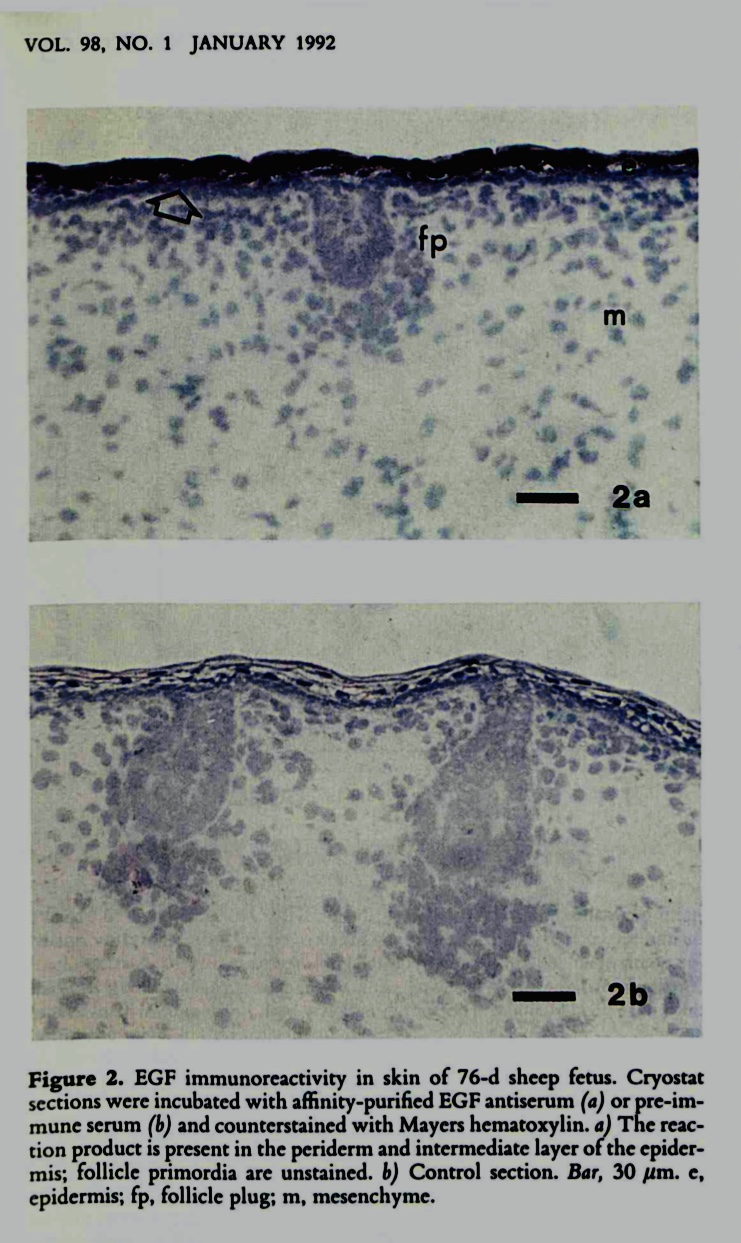
\includegraphics[width=0.9\textwidth]{image1.jpg}
  \caption{Developing follicles with associated dermal papilla cell aggregates}
  \label{fig:dpcagg}
\end{figure}

%\end{document}


In Figure~\ref{fig:dpcagg} one can see aggregates of pre-papilla cells positioned below the bulb of the developing follicle downgrowth.  In a fully developed folllicle these aggregated cells end up inside the papilla.

There may be one further cell division of the pre-papilla cells after they form an aggregate, but each aggregate is essentially a sample from a population of unaggregated pre-papilla cells. As such there is possibly sampling variation in the number of cells which form each aggregate. Such sampling variation in numbers of cells per aggregate should follow a Poisson distribution.

Given that the number of cells in each aggregate determines the base diameter of each fibre, and given that we have an empirical equation relating dermal papilla cell number to checked fibre diameter, we can investigate whether a poisson sampling of dermal papilla cell number generates a reasonable looking fibre diameter distribution.


\clearpage
\section{Materials and Methods}
The statistical language {\em R}~\cite{rprog:13} has a function {\em rpois(n,$\lambda$)} which generates {\em n} random values sampled from a Poisson distribution with parameter {\em $\lambda$}. Parameter {\em $\lambda$} is both the mean and variance. One can therefore generate a moderately large number of random poisson variates and inspect the distribution.

What we actually want is the distribution of diameter, given the Poisson simulated distribution of dermal papilla cell numbers. To get diameter distribution we transform the simulates papilla cell numbers $(C)$ to diameters $(D)$ using
\begin{displaymath}
A = 72.2312 + 3.9270C
\end{displaymath}
where $(A)$ is fibre cross sectional area, and then
\begin{displaymath}
D = \sqrt{\frac{4A}{\pi}}
\end{displaymath}
giving a set of diameters which can be displayed as a distribution.


\clearpage
\section{Results}
\subsection{Sampling considerations for pre-papilla cell aggregations}
\subsubsection{Poisson samples}
Start with two Poisson samplings of 5000 papilla cell numbers from populations with means of $50$ and $100$ papilla cells per follicle. 
\begin{verbatim}
> samp.5000.50 <- rpois(5000,50)
> samp.5000.100 <- rpois(5000,100)
> mean(samp.5000.50)
[1] 50.0694
> var(samp.5000.50)
[1] 49.84735
> mean(samp.5000.100)
[1] 99.9076
> var(samp.5000.100)
[1] 100.7876
\end{verbatim}

So 5000 would seem to be a large enough sample, the sample means are very close to the population means of $50$ and $100$.

The frequency histograms for these samples are shown in Figure~\ref{fig:dpcchist}
%\documentclass{article}
%\usepackage{graphicx,subfigure}
%\begin{document}

\begin{figure}[h]
  \centering
   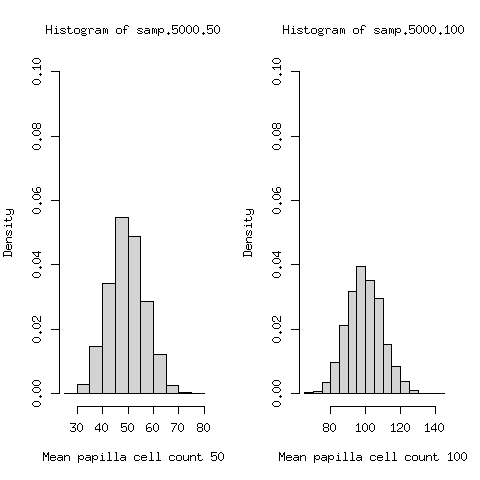
\includegraphics[width=0.9\textwidth]{dpcchist2.png}
  \caption{Histograms of papilla cell count samples from Poisson populations with means of 50 and 100 cells}
  \label{fig:dpcchist}
\end{figure}

%\end{document}


We can see that the sample with mean 100 has a larger spread ( expected because the variance is the same as the mean in Poisson populations). There is nothing else remarkable, both distributions look symmetric . The sample with mean $50$ has a slight right skew
Poisson samples with such high mean counts are expected to look symmetric like  normal distributions. Poisson samples with mean less than about 10 are markedly skewed. 

\subsubsection{Poisson sample distributions converted to diameter distributiuons}
The samples of papilla cell counts with means of 50 and 100 were converted to fibre diameter. The fibre diameter histograms are shown in Figure~\ref{fig:diamhist}
%\documentclass{article}
%\usepackage{graphicx,subfigure}
%\begin{document}

\begin{figure}[h]
  \centering
   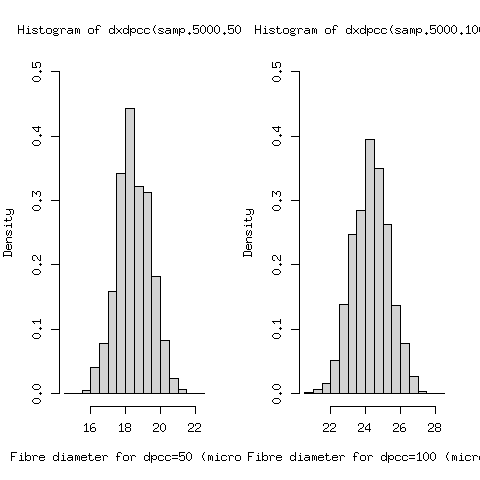
\includegraphics[width=0.9\textwidth]{diamhist2.png}
  \caption{Histograms of fibre diameter for samples of papilla cell counts from Poisson populations with means of 50 and 100 cells}
  \label{fig:diamhist}
\end{figure}

%\end{document}


The means and variances for the two histograms in Figure~\ref{fig:diamhist} are
50 cells - mean=18.4, var=0.911, 100cells - mean=24.2, var=1.066. So the variance of diameter increases with the mean. The two diameter histograms are close to symmetric. 

Note the difference in the scale for density ( the Y axis) in Figures~\ref{fig:dpcchist} and ~\ref{fig:diamhist}. This is because the widths of each frequency class are different in the two Figures. The densities sum to $1.0$ when multiplied by the class width, ie it is the area under the class intervals that sums to $1.0$.

\subsubsection{Allowing for differences in papilla cell counts between follicle types}
 From the above, it is clear that there is no way that a simple Poisson sampling for papilla cell numbers can generate a skewed fibre diameter distribution. Skewed diameter distributuons are common. We have to look elsewhere for the source of skewed diameter distributions. 

One possibility is differences in the mean papilla cell count between the various types of follicle . Pc, Pl, So, and Sd follicles tend to form a series of decreasing sizes, so there may well be larger papilla cell counts in the Pc, Pl, and So follicles, and fewer in the Sd follicles. 

We can simulate this by using the trio group modelling software (Jackson and Moore (2021)~\cite{jack:21}). This software generates a trio group of follicles and calculates their fibre diameters, starting with the following parameters
\begin{description}
\item[sositeno] number of So sites in a trio group (default 20). Pc sites are fixed at 1 and Pl sites are fixed at 2. 
\item[follinitrate] follicle initiation rate for Pc, Pl, and So follicles - ie for follicles with sites (default 4 per day per trio group)
\item[sdfollinitrate] follicle initiation rate for Sd follicles (default 8 per day). Follicles without sites initiate more rapidly.
\item[pcstarttime] day number of start of Pc initiation (default 64). 
\item[plstarttime] day number of start of Pl initiation (default 70).
\item[sostarttime] day number of start of So initiation (default 86).
\item[dayzerocellno] number of pre-papilla cells per trio group  at day zero (default 160, day zero default is day 60).
\item[pcavecellno] mean number of papilla cells aggregating at a Pc follicle site (default 65).
\item[plavecellno] mean number of papilla cells aggregating at a Pl follicle site (default 64).
\item[soavecellno] mean number of papilla cells aggregating at an So follicle site (default 59).
\item[sdavecellno] mean number of papila cells aggregating at an Sd follicle (default 53).
\item[cellbirthprob] cell birth probability for pre-papilla cell population (default 0.12)
\item[ztime] zero time for pre-papilla cell population (default day 60). 
\end{description}

There are also some parameters setting foetal growth curves. These are only used to get densities. The model runs on counts of cells and follicles. Densities are an aftercalculation.

There are a lot of parameters.  Some of them can simply be left at the default values. We might begin by looking at the result obtained by modelling one trio group with all parameters set to the above default. The model is simply a giant bookkeeping exercise tabulating each follicle as it is initiated and keeping track of differentiated and undifferentiated papilla cells. A list of all the follicles initiated in one such run is given in Table~\ref{tab:triolp}
%\documentclass{article}
%\usepackage{lscape,longtable}
%\begin{document}

% latex table generated in R 4.1.1 by xtable 1.8-4 package
% Mon Oct 18 21:00:09 2021
\label{tab:triolp}
\begin{center}
\begin{longtable}{|p{0.5in}|p{0.5in}|p{0.5in}|p{0.5in}|p{0.6in}|p{0.6in}|p{0.6in}|}
\caption{Follicle initiation table for one run of trio group simulation software
.  Parameters sositeno=10, follinitrate 4 per day, sdfollinitrate 6 per day, pcs
tarttime=64, plstarttime=70, sostarttime=86, dayzerocellno=340, pcavecellno=90,
plavecellno=89, soavecellno=62, sdavecellno=60, ztime=60} \\
  \hline
  follno & time & index & folltype & diffcellno & Diam & ppcellno\\
  \hline
\endfirsthead
\multicolumn{5}{c}%
{\tablename\ \thetable\ -- \textit{Continued from previous page}} \\
\hline
  follno & time & index & folltype & diffcellno & Diam & ppcellno \\
\hline
\endhead
\hline
\multicolumn{5}{r}{\textit{Continued on next page}} \\
\endfoot
\hline
\endlastfoot
 1.00 & 64.00 & 5.00 & Pc & 83.00 & 22.52 & 488 \\ 
 2.00 & 70.00 & 11.00 & Pl & 97.00 & 24.02 & 711 \\ 
 3.00 & 70.00 & 11.00 & Pl & 107.00 & 25.04 & 711 \\ 
 4.00 & 86.00 & 27.00 & So & 39.00 & 16.94 & 2252 \\ 
 5.00 & 86.00 & 27.00 & So & 62.00 & 20.05 & 2252 \\ 
 6.00 & 86.00 & 27.00 & So & 59.00 & 19.67 & 2252 \\ 
 7.00 & 86.00 & 27.00 & So & 54.00 & 19.03 & 2252 \\ 
 8.00 & 87.00 & 28.00 & So & 62.00 & 20.05 & 2252 \\ 
 9.00 & 87.00 & 28.00 & So & 61.00 & 19.92 & 2252 \\ 
 10.00 & 87.00 & 28.00 & So & 60.00 & 19.80 & 2252 \\ 
 11.00 & 87.00 & 28.00 & So & 50.00 & 18.49 & 2252 \\ 
 12.00 & 88.00 & 29.00 & So & 61.00 & 19.92 & 2233 \\ 
 13.00 & 88.00 & 29.00 & So & 56.00 & 19.29 & 2233 \\ 
 14.00 & 89.00 & 30.00 & Sd & 61.00 & 19.92 & 2329 \\ 
 15.00 & 89.00 & 30.00 & Sd & 85.00 & 22.74 & 2329 \\ 
 16.00 & 89.00 & 30.00 & Sd & 67.00 & 20.66 & 2329 \\ 
 17.00 & 89.00 & 30.00 & Sd & 66.00 & 20.54 & 2329 \\ 
 18.00 & 89.00 & 30.00 & Sd & 65.00 & 20.42 & 2329 \\ 
 19.00 & 89.00 & 30.00 & Sd & 64.00 & 20.30 & 2329 \\ 
 20.00 & 90.00 & 31.00 & Sd & 64.00 & 20.30 & 2143 \\ 
 21.00 & 90.00 & 31.00 & Sd & 49.00 & 18.36 & 2143 \\ 
 22.00 & 90.00 & 31.00 & Sd & 62.00 & 20.05 & 2143 \\ 
 23.00 & 90.00 & 31.00 & Sd & 69.00 & 20.90 & 2143 \\ 
 24.00 & 90.00 & 31.00 & Sd & 53.00 & 18.89 & 2143 \\ 
 25.00 & 90.00 & 31.00 & Sd & 65.00 & 20.42 & 2143 \\ 
 26.00 & 91.00 & 32.00 & Sd & 65.00 & 20.42 & 1985 \\ 
 27.00 & 91.00 & 32.00 & Sd & 63.00 & 20.17 & 1985 \\ 
 28.00 & 91.00 & 32.00 & Sd & 74.00 & 21.49 & 1985 \\ 
 29.00 & 91.00 & 32.00 & Sd & 62.00 & 20.05 & 1985 \\ 
 30.00 & 91.00 & 32.00 & Sd & 60.00 & 19.80 & 1985 \\ 
 31.00 & 91.00 & 32.00 & Sd & 64.00 & 20.30 & 1985 \\ 
 32.00 & 92.00 & 33.00 & Sd & 49.00 & 18.36 & 1786 \\ 
 33.00 & 92.00 & 33.00 & Sd & 81.00 & 22.29 & 1786 \\ 
 34.00 & 92.00 & 33.00 & Sd & 56.00 & 19.29 & 1786 \\ 
 35.00 & 92.00 & 33.00 & Sd & 75.00 & 21.61 & 1786 \\ 
 36.00 & 92.00 & 33.00 & Sd & 59.00 & 19.67 & 1786 \\ 
 37.00 & 92.00 & 33.00 & Sd & 66.00 & 20.54 & 1786 \\ 
 38.00 & 93.00 & 34.00 & Sd & 49.00 & 18.36 & 1570 \\ 
 39.00 & 93.00 & 34.00 & Sd & 59.00 & 19.67 & 1570 \\ 
 40.00 & 93.00 & 34.00 & Sd & 67.00 & 20.66 & 1570 \\ 
 41.00 & 93.00 & 34.00 & Sd & 61.00 & 19.92 & 1570 \\ 
 42.00 & 93.00 & 34.00 & Sd & 59.00 & 19.67 & 1570 \\ 
 43.00 & 93.00 & 34.00 & Sd & 71.00 & 21.14 & 1570 \\ 
 44.00 & 94.00 & 35.00 & Sd & 58.00 & 19.54 & 1353 \\ 
 45.00 & 94.00 & 35.00 & Sd & 54.00 & 19.03 & 1353 \\ 
 46.00 & 94.00 & 35.00 & Sd & 60.00 & 19.80 & 1353 \\ 
 47.00 & 94.00 & 35.00 & Sd & 54.00 & 19.03 & 1353 \\ 
 48.00 & 94.00 & 35.00 & Sd & 49.00 & 18.36 & 1353 \\ 
 49.00 & 94.00 & 35.00 & Sd & 66.00 & 20.54 & 1353 \\
 50.00 & 95.00 & 36.00 & Sd & 64.00 & 20.30 & 1141 \\ 
 51.00 & 95.00 & 36.00 & Sd & 72.00 & 21.26 & 1141 \\ 
 52.00 & 95.00 & 36.00 & Sd & 71.00 & 21.14 & 1141 \\ 
 53.00 & 95.00 & 36.00 & Sd & 67.00 & 20.66 & 1141 \\ 
 54.00 & 95.00 & 36.00 & Sd & 63.00 & 20.17 & 1141 \\ 
 55.00 & 95.00 & 36.00 & Sd & 55.00 & 19.16 & 1141 \\ 
 56.00 & 96.00 & 37.00 & Sd & 59.00 & 19.67 & 858 \\ 
 57.00 & 96.00 & 37.00 & Sd & 74.00 & 21.49 & 858 \\ 
 58.00 & 96.00 & 37.00 & Sd & 52.00 & 18.76 & 858 \\ 
 59.00 & 96.00 & 37.00 & Sd & 73.00 & 21.38 & 858 \\ 
 60.00 & 96.00 & 37.00 & Sd & 66.00 & 20.54 & 858 \\ 
 61.00 & 96.00 & 37.00 & Sd & 61.00 & 19.92 & 858 \\
 62.00 & 97.00 & 38.00 & Sd & 65.00 & 20.42 & 555 \\ 
 63.00 & 97.00 & 38.00 & Sd & 56.00 & 19.29 & 555 \\ 
 64.00 & 97.00 & 38.00 & Sd & 68.00 & 20.78 & 555 \\ 
 65.00 & 97.00 & 38.00 & Sd & 59.00 & 19.67 & 555 \\ 
 66.00 & 97.00 & 38.00 & Sd & 51.00 & 18.63 & 555 \\ 
 67.00 & 97.00 & 38.00 & Sd & 48.00 & 18.22 & 555 \\ 
 68.00 & 98.00 & 39.00 & Sd & 67.00 & 20.66 & 261 \\ 
 69.00 & 98.00 & 39.00 & Sd & 50.00 & 18.49 & 261 \\ 
 70.00 & 98.00 & 39.00 & Sd & 56.00 & 19.29 & 261 \\ 
 71.00 & 98.00 & 39.00 & Sd & 49.00 & 18.36 & 261 \\ 
 72.00 & 98.00 & 39.00 & Sd & 54.00 & 19.03 & 261 \\ 
 73.00 & 98.00 & 39.00 & Sd & 61.00 & 19.92 & 261 \\ 
   \hline
\end{longtable}
\end{center}
%\end{document}

We see 73 follicles forming one trio group listed in order of initiation.   The column {\em diffcellno} is the number of papilla cells aggregated into each follicle. This has been converted to diameter in the {\em Diam} column.  It is a fine wooled sheep with n S/P ratio of $70/3 = 23.3$. The whole process takes 35 days, from day 64 to day 98, ie initiation is completed long before birth, in this case. Pre-papilla cell numbers per trio group are shown in the column headed {\em ppcellno}. What stops the process is using up of all available pre-papilla cells. 

The diameters in Table~\ref{tab:triolp} are shown as a histogram in Figure~\ref{fig:onetriodiamhist}
%\documentclass{article}
%\usepackage{graphicx,subfigure}
%\begin{document}

\begin{figure}[h]
  \centering
   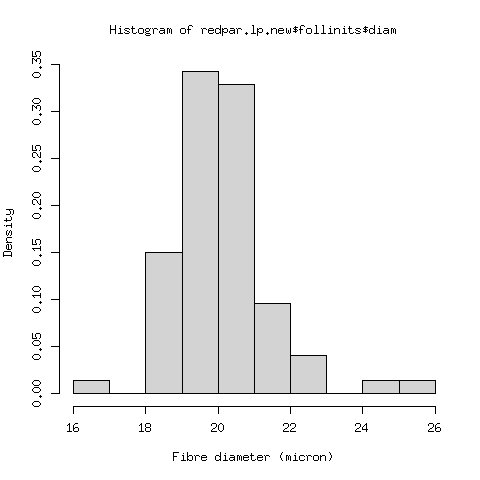
\includegraphics[width=0.9\textwidth]{onetriogpdiam.png}
  \caption{Histogram of fibre diameter for the  one trio group in Table~\ref{tab:triodefault}}
  \label{fig:onetriodiamhist}
\end{figure}

%\end{document}


This distribution has some skew due to the coarseer diameters of primary fibres. 
However a trio group is only about 100 follicles ( in the above case 73). We need to run the model about 50 times - ie generate 50 trio groups , and pool the resultant follicle papilla cell numbers, and fibre diameters. 

\subsubsection{More than one trio group}
We ran the {\em trio()} modelling software 50 times and pooled the diameters of all fibres from all follicles initiated in all trio groups. The histogram of these diameters is shown in Figure~\ref{fig:diamhist50}
%\documentclass{article}
%\usepackage{graphicx,subfigure}
%\begin{document}

\begin{figure}[h]
  \centering
   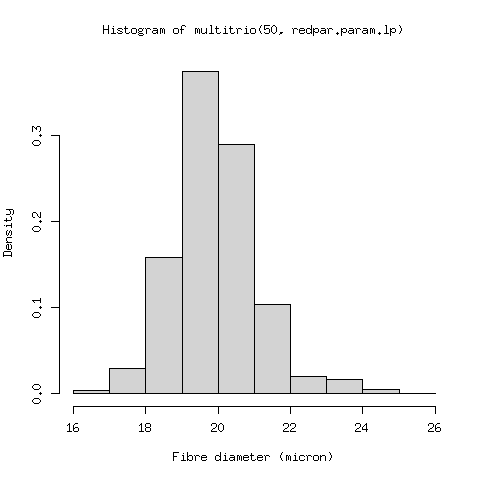
\includegraphics[width=0.9\textwidth]{diamhist50.png}
  \caption{Histogram of fibre diameter for 50 trio groups modelled with the {\em trio()} software with the same parameters as Table~\ref{tab:triolp}}
  \label{fig:diamhist50}
\end{figure}

%\end{document}


This now looks very much like a typical Merino fibre diameter distribution for a single sheep.  A sample from a bale might look different, because it would include variation between fleeces.

We ran the {\em trio()} modelling software again, this time setting the numbers of papilla cells per follicle to Pc=160, Pl=150, So=40, Sd=35, to simulate a primitive 2-coated fleece. The resultin histogram, from 50 trio groups is shown in Figure~\ref{fig:diamhistprimitive}.
%\documentclass{article}
%\usepackage{graphicx,subfigure}
%\begin{document}

\begin{figure}[h]
  \centering
   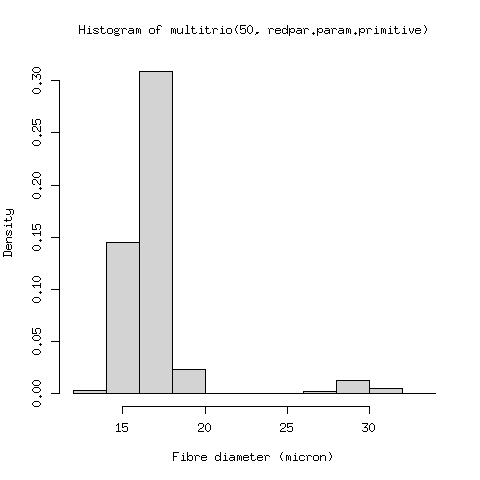
\includegraphics[width=0.9\textwidth]{diamhistprimitive.png}
  \caption{Histogram of fibre diameter for 50 trio groups modelled with the {\em trio()} software with the same parameters as Table~\ref{tab:triolp} except papilla cells per follicle altered to Pc=160, Pl=150, So=40, Sd=35 to simulate a primitive 2-coated fleece}
  \label{fig:diamhistprimitive}
\end{figure}

%\end{document}


This diameter distribution is rather like that of a primitive sheep, for example those shown by Ryder(1984)~\cite{ryde:84} The diameters of primary fibres might have been set larger, ie more papilla cells per primary follicle.


\subsection{Comparing simulated with actual fibre diameter distributions}
Some data from CSIRO genetic research flocks is available with fibre diameter distribution measured on skin sections and an associated follicle density and S/P ratio measured on the same section. The animals were Merino of medium to fine diameter sampled at 18 months of age. We chose a number of sheep representing the range of variation in these flocks, and attempted to simulate the fibre diameter distribution of each starting with values for Dp, Ds, converted to Pc,Pl,So,Sd papilla cell numbers, and with the other starting parameters permuted to attempt to get a matching distribution , and a matching S/P ratio.

\clearpage
\section{Discussion}
Our thesis is that most of the variation in diameter between fibres within a sheep is controlled by a random sampling of dermal papilla cell numbers forming aggregates. That is , it is not controlled at all, it is chance variation. We emulate this with sampling from a Poisson distribution.

However there is a small amount of fibre diameter variation that is due to systematic differences in dermal papilla cell number between follicle types (Pc, Pl, So, Sd) within a sheep. This variation is under genetic control, and is what is responsible for skewed within sheep fibre diameter distributions. We have ben able to show that one can simulate fibre diameter distributions with skewness or bimodality, simply by allocating more dermal papilla cells to the earliwer forming follicle types (Pc, Pl, So).

It may be that instead of making follicle types, the most realistic strategy may be to allocate dermal papilla cell numbers to follicles according to their time of initiation. The effect on diameter distribution would be similar. We have not tried this approach, but it may be more biologically meaningful.

We are trying to cope with the issue of while we are sure that dermal papilla cell number controls maximim or potential or base diameter ( actually cross sectional area) , all our data are of {\em checked} diameter, ie what the follicles grow when they have to share a limited nutrient supply among all the follicles in a trio group.

Some data on changes in diameter along staples (staple diameter profiles) give a view of how much the {\em check} effect can vary over time, at least in so far as mean diameter is concerned. What we really need to know is how {\em check} effects affect diameter distribution.
\clearpage
\begin{thebibliography}{}

\bibitem{bogo:40}
 Bogolyubsky S.N. (1940) cited by Fraser A.S and Short B.F. (1960) The Biology of the Fleece. Animal Research Laboratories Technical Paper No 3. CSIRO Melbourne 1960.


\bibitem{cart:43}
Carter H.B. (1943) Studies in the biology of the skin and fleece of sheep. 1. The development and general histology of the follicle group in the skin of the Merino. 2. The use of tanned sheepskin in the study of follicle population density. 3. Notes on the arrangement, nomenclature, and variation of skin folds and wrinkles in the Merino. C.S.I.R. Bulletin No 164, Melbourne, 1943

\bibitem{cart:55}
Carter, H.B. (1955) The hair follicle group in sheep Animal Breeding Abstracts 23(2) 101-116

\bibitem{cart:68}
Carter,H.B. (1968) Comparative Fleece Analysis Data for Domestic Sheep. The Principal Fleece Staple Values of Some Recognised Breeds. Agricultural Research Council, 1968

\bibitem{chi:13}
Chi, W., Wu, E., and MOrgan, B.A. (2013) Dermal papilla cell number specifies hair size shape and cycling and its reduction causes follicular decline. Development 140(8):1676-1683

\bibitem{down:75}
Downes, A. M., Jackson, N. and Griffiths, D. A. (1975) Measurement of mean fibre diameter and colour quenching of wool samples by liquid scintillation spectrometry. 5th Int. Wool Text. Res. Conf. Aachen, Germany.

\bibitem{fras:60}
Fraser A.S and Short B.F. (1960) The Biology of the Fleece. Animal Research Laboratories Technical Paper No 3. CSIRO Melbourne 1960.

\bibitem{gord:08}
Gordon-Thompson, C., Botto, S.A., Cam, G.R., and Moore, G.P.H. (2008) Notch pathway gene expression and wool follicle cell fates. Aust. J. Exp. Agric. 48(5) 648-656

\bibitem{hard:56}
Hardy, M.H. and Lyne, A.G. (1956) The prenaltal development of wool follicles in Merino sheep. Aust. J. Biol. Sci. 9:423-441

\bibitem{jack:79}
Jackson, N. and Downes, A. M. (1979) The fibre diameter profile of wool staples from individual sheep. Aust. J. agric. Res. 30:163-171

\bibitem{jack:17}
Jackson, N. (2017) Genetics of primary and secondary fibre diameters and densities in Merino sheep. URL https://github.com/nevillejackson/atavistic-sheep/mev-rewrite/supplementary/genetic-parameters/psparam.pdf

\bibitem{jack:17a}
Jackson, N. (2017) Genetic relationship between skin and wool traits in Merino sheep. Part I Responses to selection and estimates of genetic parameters. URL https://github.com/nevillejackson/Fleece-genetics/tree/master/skinandfleeceparameters/ab3220/skinwool1.pdf

\bibitem{jack:17b}
Jackson, N. (2017) What are the defining characteristics of a primitive sheep relative to a Modern Merino sheep.  URL https://github.com/nevillejackson/atavistic-sheep/tree/master/mev-rewrite/supplementary/primitive/primitive.pdf

\bibitem{jack:18}
Jackson, N., Swan, P.G.S. and Watts, J.E. (2018) Questions regarding developmental control of fibre diameter and fibre length growth rate in sheep. URL https://github.com/nevillejackson/Fleece-biology/tree/master/diamlen/diamlen.pdf

\bibitem{jack:21}
Jackson, N. and Moore, G.P.M. (2021) Modelling trio group formation from a population of pre-papilla cells. Unfinished work.

\bibitem{jack:90}
Jackson, N., Maddocks, I.G., Lax, J., Moore, G.P.M. and Watts, J.E. (1990) Merino Evolution, Skin Characteristics, and Fleece Quality. URL https://github.com/nevillejackson/atavistic-sheep/mev/evol.pdf 

\bibitem{jack:18a}
Jackson, N. and Moore, G.P.H. (2018) R package {\em ppcell}. URL

\bibitem{madd:88}
Maddocks, I.G. and Jackson, N. (1988) Structural studies of sheep, cattle, and goat skin. CSIRO, Division of Aimal Production, Sydney.

\bibitem{metc:62}
Metcalf, J., Meschia, G., Hellegers, A., Prytowsky, H., Huchabee, W., and Barron, D.H. (1962) Observations on the growth rates and organ weights of fetal sheep at altitude and sea level. Quart. J. exp. Physiol. XLVII (4) 305-313

\bibitem{moor:84}
Moore G.P.M. and Jackson, N. (1984) An hypothesis implicating a founder cell population in the regulation of wool follicle formation and distribution in sheep skin. J. Embryol. Exp. Morph. 82 (Suppl), 259

\bibitem{moor:89}
Moore G.P.M., Jackson, N., and Lax, J. (1989) Evidence of a unique developmental mechanism specifying both wool follicle density and fibre size in sheep selected for single skin and fleece characters. Genet. Res. Camb. 53:57-62

\bibitem{moor:98}
Moore, G.P.M., Jackson, N., Isaacs, K., and Brown, G (1998) J. Theoretical Biology 191:87-94

\bibitem{rprog:13}
R Core Team (2013). R: A language and environment for statistical
  computing. R Foundation for Statistical Computing, Vienna, Austria.
  ISBN 3-900051-07-0, URL http://www.R-project.org/.

\bibitem{ryde:84}
Ryder, M. L. (1984) Medieval Sheep and Wool Types.  Agricultural History Review 32:14-28

\bibitem{ryde:68}
Ryder, M.L. and Stevenson, S.K.(1968) Wool Growth. Academic Press, London.

\bibitem{swan:21}
Swan, P. G., Jackson, N. and Moore, P, G. M. (2021) Dermal papilla sell counts and fibre diameter. URL  not there yet!

\bibitem{tapl:62}
Taplan, D.E., and Everitt, G.C. (1962) The influence of prenatal nutrition on postnatal performance of Merino lambs. Waite Agricultural Research Institute, University of Adelaide: 72-81
URL https://pdfs.semanticscholar.org/90b6/
db6e9763d25add182220c0b369023072d41b.pdf

\bibitem{turn:70}
Turner, H.N., Brooker, M.G. and Dolling, C.H.S(1970) Response to selection in Australian Merino sheep. III Single character selection for high and low values of clean wool weight and its components. Aust. J. agric. Res. 21:955-984

\bibitem{watt:18}
Watts, J.E., and Jackson, N. (2018) Is collagen quantity and properties involved in wrinkle formation and/or in follicle development? URL https://github.com/nevillejackson/SRS-Merino/tree/master/supplementary/collagen/collagen.pdf

\bibitem{xavi:03}
Xavier, S.P., Gordon-Thomson, C. Wynn, P.C., McCullagh, P., Thomson, P.C., Tomkins, L., Mason, R.S., and Moore, G.P.M.(2003) Evidence that Notch and Delta expressions have a role in dermal condensate aggregation during wool follicle initiation. Experimental Dermatology, 22:656-681

\end{thebibliography}

\appendix
\section{Appendix}
The raw data are listed here for completeness
\end{document}
